% Bachelorarbeit — claude-tunnel
% HAW Hamburg, Fakultät Technik und Informatik, Department Informatik.
% Build (Docker-only): scripts/thesis-build.sh  →  docs/thesis/thesis.pdf
\documentclass[12pt,a4paper,oneside,bibliography=totoc,listof=totoc,parskip=half]{scrbook}

% --- Sprache & Kodierung ---
\usepackage[utf8]{inputenc}
\usepackage[T1]{fontenc}
\usepackage[ngerman,english]{babel}
\usepackage{csquotes}
\usepackage{amsmath}

% --- Layout & Grafik ---
\usepackage[a4paper,margin=3cm,bindingoffset=1cm]{geometry}
\usepackage{graphicx}
\graphicspath{{data/}}
\usepackage{booktabs}
\usepackage{lmodern}
\usepackage{tikz}
\usetikzlibrary{arrows.meta,positioning}
\usepackage{listings}
\lstset{basicstyle=\ttfamily\footnotesize, breaklines=true, frame=single,
        columns=fullflexible, keepspaces=true, showstringspaces=false,
        captionpos=b, xleftmargin=0.5em}

% --- Literatur ---
\usepackage[backend=biber,style=numeric,sorting=nyt]{biblatex}
\addbibresource{references.bib}

% --- Verweise (zuletzt laden) ---
\usepackage[hidelinks]{hyperref}

% --- Metadaten (Platzhalter, vor Abgabe ausfüllen) ---
\newcommand{\arbeittitel}{Zero-Knowledge-Netzwerktunnel für zensurresistente Kommunikation}
\newcommand{\arbeituntertitel}{Entwurf, Implementierung und emulationsbasierte Evaluation}
\newcommand{\autorname}{Vorname Nachname}
\newcommand{\matrikelnr}{0000000}
\newcommand{\erstgutachter}{Prof.\ Dr.\ Erstgutachter}
\newcommand{\zweitgutachter}{Prof.\ Dr.\ Zweitgutachter}
\newcommand{\abgabedatum}{TT.\,MM.\,JJJJ}

\begin{document}
\selectlanguage{ngerman}
\frontmatter

% ===================== Titelblatt =====================
\begin{titlepage}
  \centering
  {\large Hochschule für Angewandte Wissenschaften Hamburg\par}
  {\large Fakultät Technik und Informatik\par}
  {\large Department Informatik\par}
  \vfill
  {\Large\bfseries \arbeittitel\par}
  \vspace{0.5em}
  {\large \arbeituntertitel\par}
  \vspace{2em}
  {\large Bachelorarbeit\par}
  \vfill
  \begin{tabular}{rl}
    Vorgelegt von: & \autorname \\
    Matrikelnummer: & \matrikelnr \\[1em]
    Erstgutachter: & \erstgutachter \\
    Zweitgutachter: & \zweitgutachter \\[1em]
    Abgabedatum: & \abgabedatum \\
  \end{tabular}
  \vfill
\end{titlepage}

% ===================== Eidesstattliche Erklärung =====================
\chapter*{Eidesstattliche Erklärung}
\thispagestyle{plain}
Hiermit versichere ich an Eides statt, dass ich die vorliegende Bachelorarbeit
mit dem Titel \enquote{\arbeittitel} selbstständig und ohne fremde Hilfe
verfasst und keine anderen als die angegebenen Quellen und Hilfsmittel benutzt
habe. Die Stellen der Arbeit, die dem Wortlaut oder dem Sinn nach anderen Werken
entnommen sind, wurden unter Angabe der Quelle kenntlich gemacht. Diese Arbeit
hat in gleicher oder ähnlicher Form noch keiner Prüfungsbehörde vorgelegen.
\par\vspace{3em}
\noindent Hamburg, den \abgabedatum \hfill\rule{6cm}{0.4pt}\\
\hspace*{\fill}\autorname

% ===================== Kurzfassung / Abstract =====================
\chapter*{Kurzfassung}
Diese Arbeit entwirft und implementiert einen \emph{Zero-Knowledge-Netzwerktunnel}
für zensurresistente Kommunikation: ein providerblindes Relay, das nur
Chiffretext weiterleitet, während die Ende-zu-Ende-Verschlüsselung zwischen
Client und Ursprung über das Noise-Protokoll erfolgt. Der Zugang zum Relay wird
über ein Proof-of-Work-gestütztes Rendezvous und tokenbasierte Ratenbegrenzung
geschützt. Der Prototyp ist in Rust auf Basis von QUIC umgesetzt und wird in
einem Docker-basierten Testbett unter emulierten Netzbedingungen
(\texttt{tc netem}) auf seine Roundtrip-Latenz hin evaluiert.

\begin{otherlanguage}{english}
\chapter*{Abstract}
This thesis designs and implements a \emph{zero-knowledge network tunnel} for
censorship-resistant communication: a provider-blind relay that forwards only
ciphertext, while end-to-end encryption between client and origin is provided by
the Noise protocol. Access to the relay is guarded by a proof-of-work
rendezvous and per-token rate limiting. The prototype is implemented in Rust on
top of QUIC and evaluated for round-trip latency in a Docker-based testbed under
emulated network conditions (\texttt{tc netem}).
\end{otherlanguage}

\tableofcontents

% ===================== Hauptteil =====================
\mainmatter
\chapter{Einleitung}
\label{ch:einleitung}

\section{Motivation und Problemstellung}
\label{sec:motivation}

Dienste hinter NAT oder Firewalls für entfernte Nutzer erreichbar zu machen,
ist ein alltäglicher Bedarf; die verbreiteten Tunneldienste lösen ihn jedoch um
den Preis des Vertrauens: Der Verkehr wird beim Anbieter terminiert, sodass
dieser den Klartext einsehen und die Verbindung auf Zuruf kappen kann. Für
Nutzer mit einem Schutzbedarf gegen Zensur ist ein Anbieter, der den Datenverkehr
\emph{sehen} oder \emph{unterbrechen} kann, jedoch selbst ein Angriffspunkt.

Diese Arbeit verfolgt den entgegengesetzten Entwurf: einen
\emph{providerblinden} (zero-knowledge) Tunnel, bei dem der Betreiber
bewusst aus drei Dingen herausgehalten wird -- dem \emph{Inhalt} (die
Nutzlast-Verschlüsselung terminiert erst am kundeneigenen Origin, nie beim
Betreiber), dem \emph{Vertrauen} (die Schlüssel sind kundenverankert, es gibt
keine betreiberseitige PKI) und, soweit möglich, dem \emph{Datenpfad} selbst.
Die Zero-Knowledge-Eigenschaft ist dabei bewusst auf die \emph{Nutzlast}
begrenzt: Strukturelle Metadaten wie die Existenz eines Tunnels oder -- im
Relay-Fall -- grobe Zeit- und Volumenzähler bleiben sichtbar. Durchsetzung
reduziert sich auf einen einzigen, groben Hebel (Terminierung eines Tokens),
der nur an einer eng definierten \emph{rechtlichen Grenze} greift.

Aus dieser Haltung ergibt sich ein Spannungsfeld: Providerblindheit und
Zensurresistenz erkauft man sich mit zusätzlichen Vermittlungsschritten
(Rendezvous, Relay) und kryptographischem Aufwand. Ob und in welchem Umfang
diese Schutzziele die Latenz eines Tunnels belasten, ist die zentrale empirische
Frage dieser Arbeit.

\section{Zielsetzung}
\label{sec:zielsetzung}

Ziel der Arbeit ist der Entwurf, die prototypische Implementierung und die
emulationsbasierte Evaluation eines solchen Tunnels. Der Prototyp ist in Rust auf
Basis von QUIC umgesetzt und realisiert den providerblinden Relay-Pfad
Client~$\rightarrow$~Edge~$\rightarrow$~Agent~$\rightarrow$~Origin mit einem
Proof-of-Work-gestützten, ratenbegrenzten Rendezvous. Die Noise-basierte
Ende-zu-Ende-Verschlüsselung ist als kryptographischer Baustein umgesetzt. Die
Bewertung erfolgt in einem vollständig Docker-basierten Testbett, in dem
Netzbedingungen (Verzögerung, Paketverlust, Bandbreite) mit \texttt{tc netem}
emuliert und die Roundtrip-Latenz reproduzierbar vermessen werden.

\section{Forschungsfragen}
\label{sec:forschungsfragen}

Die Arbeit gliedert sich an drei Forschungsfragen:

\begin{description}
  \item[FF1 -- Realisierbarkeit.] Lässt sich ein providerblinder,
    zensurresistenter Tunnel aus etablierten Bausteinen -- QUIC als Transport,
    Noise für die Ende-zu-Ende-Sicherheit, Proof-of-Work als Zugangsschutz --
    schlüssig entwerfen und implementieren?
  \item[FF2 -- Latenz-Overhead.] Welchen Grund-Overhead verursacht der
    providerblinde Vermittlungspfad (Verbindungsaufbau, PoW-Rendezvous,
    Mehrsprung-Relay) gegenüber einer direkten Verbindung?
  \item[FF3 -- Verhalten unter Netzbedingungen.] Wie skaliert die
    Tunnel-Roundtrip-Latenz mit Netzverzögerung und Paketverlust?
\end{description}

\section{Aufbau der Arbeit}
\label{sec:aufbau}

Kapitel~\ref{ch:grundlagen} führt die technischen Grundlagen ein
(providerblinde Relays, Noise, QUIC, Proof-of-Work). Kapitel~\ref{ch:architektur}
beschreibt den Systementwurf und dessen Entwurfsentscheidungen.
Kapitel~\ref{ch:implementierung} dokumentiert die Umsetzung des Prototyps.
Kapitel~\ref{ch:evaluation} stellt das Testbett und die Messergebnisse vor und
beantwortet FF2 und FF3. Kapitel~\ref{ch:fazit} fasst die Ergebnisse zusammen
und gibt einen Ausblick auf die offenen Punkte.

\chapter{Grundlagen}
\label{ch:grundlagen}

Dieses Kapitel führt die technischen Grundlagen ein und wird in Paket~M7.2
ausgearbeitet: Zero-Knowledge- bzw.\ providerblinde Relays, das
Noise-Protokoll~\cite{noiseprotocol} (Handshake \texttt{Noise\_IK}), QUIC als
Transport~\cite{rfc9000,rfc9001} sowie Proof-of-Work als
Zugangsschutz~\cite{back2002hashcash}.

\chapter{Verwandte Arbeiten}
\label{ch:relatedwork}

Dieses Kapitel ordnet \texttt{claude-tunnel} in bestehende Systeme ein und
schärft die zentrale Unterscheidung der Arbeit heraus: die
\emph{Providerblindheit}. Betrachtet werden vier Familien verwandter Systeme ---
klassische VPNs (Abschnitt~\ref{sec:rw-vpn}), Reverse-Tunnel-Dienste
(Abschnitt~\ref{sec:rw-reverse}), Anonymitäts- und Zensurumgehungssysteme
(Abschnitt~\ref{sec:rw-anon}) sowie QUIC-basierte Relays
(Abschnitt~\ref{sec:rw-quic}). Der abschließende Abschnitt~\ref{sec:rw-abgrenzung}
verdichtet die Abgrenzung in einer Gegenüberstellung. Leitfrage ist durchgehend:
\emph{Wer terminiert die Verschlüsselung, und wer kann folglich Klartext lesen
oder die Verbindung kappen?}

\section{Klassische VPNs und WireGuard}
\label{sec:rw-vpn}

Klassische VPNs stellen einen verschlüsselten Tunnel zwischen zwei Endpunkten
her. Bei WireGuard~\cite{donenfeld2017wireguard} etwa terminiert die Verschlüsselung an den beiden Peers
selbst: Der Tunnel verbindet einen Client mit einem Server, der zugleich
Gegenstelle und Vertrauensanker ist. Für den hier verfolgten Anwendungsfall ---
ein kundeneigenes Origin hinter einer restriktiven Netzgrenze ohne öffentliche
Adresse erreichbar zu machen --- ist dieses Modell nur bedingt geeignet: Es
existiert kein providerblindes \emph{Relay} zwischen den Parteien, das Verkehr
vermittelt, ohne selbst Endpunkt zu sein. Wer einen VPN-Server als
Vermittlungsknoten betreibt, terminiert dessen Verschlüsselung und sieht den
weitergeleiteten Verkehr im Klartext. WireGuard löst die Transport- und
Schlüsselfrage elegant, adressiert aber gerade nicht die Trennung von blinder
Vermittlung und kundenseitig verankerter Ende-zu-Ende-Sicherheit, die den Kern
dieser Arbeit bildet. \texttt{claude-tunnel} übernimmt die Idee moderner,
schlanker Handshakes --- die Datenebene nutzt Noise~\cite{noiseprotocol} ---,
verschiebt die Terminierung jedoch vom Vermittler an das kundeneigene Ziel.

Näher am hier verfolgten Ansatz als das klassische VPN liegen jüngere Overlay-
und Secure-Channel-Systeme, deren Vermittler den Nutzlast-Schlüssel bewusst nicht
halten. Nebula~\cite{nebula} spannt ein Noise-basiertes Mesh zwischen
authentifizierten Hosts auf, in dem koordinierende \emph{Lighthouses} die Peers
zusammenführen, ohne die Ende-zu-Ende-Sitzung zu terminieren. Tailscale reicht
Verkehr, wenn kein direkter Pfad zustande kommt, über verschlüsselte
\emph{DERP}-Relays weiter, die die WireGuard-Pakete lediglich
durchreichen~\cite{tailscalederp}; die zugehörige Steuerebene lässt sich mit
Headscale~\cite{headscale} selbst betreiben. Ockam~\cite{ockam} wiederum baut
mehrsprüngige, gegenseitig authentifizierte Ende-zu-Ende-Kanäle, deren Relays
als Architektur-Eigenschaft ausschließlich Chiffretext weiterleiten. Diese
Systeme zeigen, dass \emph{payload-blindes Relaying} für sich genommen kein
Alleinstellungsmerkmal ist, sondern verbreitete Praxis. Der Beitrag dieser Arbeit
liegt daher nicht in der Nutzlast-Blindheit allein, sondern in ihrer Kombination
mit einem opaken Routing-Token (das zusätzlich das Vermittlungsziel verbirgt),
einem KYC-freien Proof-of-Work-Rendezvous und kundenverankerten Noise-Schlüsseln
ohne zentrale PKI (Abschnitt~\ref{sec:rw-abgrenzung}).

\section{Reverse-Tunnel-Dienste}
\label{sec:rw-reverse}

Reverse-Tunnel-Dienste wie Cloudflare Tunnel~\cite{cloudflaretunnel},
ngrok~\cite{ngrok} oder Tailscale Funnel~\cite{tailscalefunnel} lösen
dieselbe Erreichbarkeitsaufgabe: Ein Agent im privaten Netz baut eine
ausgehende Verbindung zu einer Anbieter-Infrastruktur auf, über die eingehender
Verkehr an das interne Ziel zurückgereicht wird. Damit entfällt die
Notwendigkeit eingehender Firewall-Freigaben. Entscheidend für die Abgrenzung ist
jedoch, \emph{wo die Transport\-verschlüsselung terminiert}: Bei diesen Diensten
endet die TLS-Sitzung beim Anbieter. Der Betreiber steht als vollwertiger
Man-in-the-Middle im Pfad, sieht den Klartext des vermittelten Verkehrs und kann
einzelne Tunnel jederzeit inhaltlich inspizieren oder kappen. Adressiert werden
die Tunnel überdies typischerweise über öffentliche Hostnamen, deren Zuordnung
der Anbieter kennt und kontrolliert.

Genau dieses Vertrauensmodell ist das \emph{Gegenmodell} zu \texttt{claude-tunnel}.
Der providerblinde Ansatz kehrt die Eigenschaft um: Das Relay leitet
ausschließlich Chiffretext weiter, hält keinen Schlüssel zur Nutzlast und
adressiert Tunnel nicht über einen Hostnamen, sondern über ein opakes
\emph{Routing-Token} ohne SNI-Information. Der Betreiber bleibt damit von Inhalt
und Vermittlungsziel abgeschnitten und ist als Druck- oder Zensurpunkt entwertet
--- die funktionale Bequemlichkeit des Reverse-Tunnels wird ohne die
Vertrauensbürde des klartextsichtigen Anbieters erreicht.

\section{Anonymität und Zensurumgehung}
\label{sec:rw-anon}

Tor~\cite{dingledine2004tor} und allgemeiner das Onion-Routing verfolgen ein anderes Bedrohungsmodell:
Ziel ist die \emph{Anonymität} der kommunizierenden Parteien, erreicht durch
mehrstufige, geschichtete Verschlüsselung über mehrere unabhängige Relays, sodass
kein einzelner Knoten Sender und Empfänger zugleich kennt. \emph{Pluggable
transports} wie obfs4~\cite{obfs4} oder Shadowsocks~\cite{shadowsocks} ergänzen dies um Verschleierung des
Verkehrsmusters, um Deep-Packet-Inspection und Protokollfilter zu unterlaufen.
Weitere Umgehungsansätze verlagern die Resistenz in die Netzinfrastruktur ---
etwa Domain Fronting~\cite{fifield2015domainfronting}, das Sperren durch
Mitnutzung großer, nicht blockierbarer Fronting-Domains unterläuft, oder
Refraction-/Decoy-Routing wie Telex~\cite{wustrow2011telex}; Messplattformen wie
OONI~\cite{filasto2012ooni} dokumentieren Verbreitung und Methodik solcher
Blockaden empirisch. Diese Systeme schützen also primär die \emph{Identität} und
die \emph{Beobachtbarkeit} der Kommunikation gegenüber Netzbeobachtern.

\texttt{claude-tunnel} zielt demgegenüber nicht auf Anonymität, sondern auf
\emph{Providerblindheit}: Der Betreiber darf durchaus wissen, \emph{dass} ein
Tunnel existiert und grobe Zeit- und Volumenzähler sehen --- er darf nur die
Nutzlast weder lesen noch das Origin-Schlüsselmaterial erlangen. Die
Bedrohungsmodelle sind damit komplementär, nicht deckungsgleich. Verwandt bleiben
gleichwohl die Fragen der \emph{Metadaten}-Minimierung (welche strukturellen
Spuren ein Vermittler zwangsläufig sieht) und der \emph{Denial-of-Service}-
Resistenz eines offenen, KYC-freien Zugangs. Wo Tor auf Netzwerk- und
Reputationsmechanismen setzt, verwendet \texttt{claude-tunnel} ein
Proof-of-Work-Rendezvous~\cite{back2002hashcash} mit tokenweiser Ratenbegrenzung
als primären Sybil-~\cite{douceur2002sybil} und Flutungs-Schutz.

\section{QUIC-Relays und MASQUE}
\label{sec:rw-quic}

Auf der Transportebene ist \texttt{claude-tunnel} den QUIC-basierten
Relay-Ansätzen verwandt. QUIC~\cite{rfc9000} bündelt Verbindungsaufbau,
Verschlüsselung und Multiplexing über UDP und eignet sich damit für den
schnellen Aufbau vieler kurzlebiger Tunnel; die Vertraulichkeit ruht dabei auf
TLS~1.3~\cite{rfc8446}, das QUIC in seinen Handshake integriert. Das
MASQUE-Framework~\cite{rfc9298,rfc9484} baut auf QUIC
und HTTP/3 auf, um Proxy- und Tunneldienste über eine QUIC-Verbindung zu
transportieren --- konzeptionell ein Relay, das UDP- oder IP-Verkehr für einen
Client weiterreicht. Die Datenebene dieser Arbeit teilt diese Transportbasis:
QUIC (via \texttt{quinn}) ist der primäre Transport, ergänzt um einen
TLS-über-TCP-Rückfall für Umgebungen, in denen UDP blockiert ist.

Der Unterschied liegt erneut in der Terminierung und der Schlüsselverankerung:
Ein MASQUE-Proxy terminiert die QUIC-Verbindung des Clients bei sich und ist
somit prinzipiell klartextsichtig auf der Proxy-Sitzung. \texttt{claude-tunnel}
legt über den QUIC-Transport eine zweite, providerblinde Schicht: eine
Ende-zu-Ende-Noise-Sitzung zwischen Client und Origin, deren Chiffretext das
Relay lediglich durchreicht. Der Transport ist verwandt; das Vertrauensmodell ist
es nicht.

\section{Abgrenzung}
\label{sec:rw-abgrenzung}

Tabelle~\ref{tab:rw-abgrenzung} stellt die vier Familien anhand der
entscheidenden Merkmale gegenüber. Der Unterschied bündelt sich in einer Zeile:
Bei WireGuard, Cloudflare Tunnel und Tor liegt die für den Nutzlastschutz
relevante Terminierung entweder beim Vermittler oder ist gar nicht als blindes
Relay konzipiert; nur \texttt{claude-tunnel} verbindet ein nutzlast-blindes Relay
mit einer kundenseitig am Origin verankerten Terminierung.

\begin{table}[t]
\centering
\caption{Abgrenzung entlang von Terminierung, Klartextsicht, Kappbarkeit und
Adressierung.}
\label{tab:rw-abgrenzung}
\begin{tabular}{llll}
\toprule
Eigenschaft & WireGuard & Cloudflare Tunnel & Tor \\
\midrule
Wer terminiert TLS/Krypto & Peer/Server & Anbieter & Origin (mehrfach) \\
Wer sieht Klartext & Server-Peer & Anbieter & kein Einzelknoten \\
Wer kann kappen & Server-Peer & Anbieter & jedes Relay (Pfad) \\
Öffentl. Hostname nötig & Server-Endpunkt & ja & nein \\
\bottomrule
\end{tabular}
\end{table}

Die konzeptionell nächsten Vorläufer sind nicht die klassischen Tunnel, sondern
jüngere Ansätze, die das \emph{Wissen} über eine Verbindung bewusst auf mehrere
Parteien aufteilen. Oblivious HTTP~\cite{rfc9458} trennt den Anfrageinhalt von
der Absenderidentität: Ein Relay verbirgt die Client-Adresse, während ein Gateway
die Anfrage entschlüsselt und an das Ziel weiterreicht. Damit sieht der Gateway
sehr wohl Ziel und Klartext, und das Modell ist auf einzelne, zustandslose
HTTP-Anfragen zugeschnitten statt auf einen langlebigen, protokollagnostischen
Tunnel. Apples iCloud Private Relay~\cite{appleprivaterelay} nutzt zwei Hops mit
Ingress-/Egress-Trennung, sodass kein einzelner Betreiber zugleich Client-IP und
Zieladresse kennt; die Trennung ruht jedoch auf \emph{zwei getrennten
Betreiberrollen}, und die Sitzung zum Ziel terminiert regulär --- eine
kundenseitig verankerte Nutzlast-Blindheit gegenüber einem \emph{einzelnen}
Vermittler ist damit nicht gegeben. \texttt{claude-tunnel} grenzt sich gegen
beide dadurch ab, dass ein \emph{einzelner} Betreiber weder Nutzlast noch
Vermittlungsziel erfährt --- Chiffretext statt Klartext, opakes Routing-Token
statt Hostname --- und die Terminierung unabhängig von einer
Zwei-Parteien-Aufteilung am kundeneigenen Origin verankert bleibt.

Die Alleinstellung von \texttt{claude-tunnel} ergibt sich aus der Kombination
vierer Bausteine, die in dieser Zusammenstellung bei keinem der verglichenen
Systeme --- auch nicht bei diesen nächsten Vorläufern --- auftritt:

\begin{itemize}
  \item ein \emph{nutzlast-blindes Relay}, das ausschließlich Chiffretext
    weiterleitet und keinen Schlüssel zur Nutzlast besitzt;
  \item ein \emph{opakes Routing-Token} statt eines Hostnamens, das dem
    Betreiber auch das Vermittlungsziel verbirgt (keine SNI- oder
    Hostnamen-Information);
  \item ein \emph{Proof-of-Work-Rendezvous} mit tokenweiser Ratenbegrenzung als
    KYC-freier Zugangs- und DoS-Schutz~\cite{back2002hashcash};
  \item \emph{kundenseitig verankerte Noise-Schlüssel ohne
    PKI}~\cite{noiseprotocol} --- die Ende-zu-Ende-Sicherheit terminiert am
    kundeneigenen Origin und benötigt weder eine Zertifikatshierarchie noch einen
    anbieterseitigen Vertrauensanker.
\end{itemize}

Für \texttt{claude-tunnel} bedeutet dies: Die funktionale Erreichbarkeit eines
Reverse-Tunnels wird mit dem Vertrauensmodell eines providerblinden Relays
zusammengeführt --- der Betreiber vermittelt, ohne Endpunkt oder Vertrauensanker
zu sein.

\chapter{Anforderungen}\label{ch:anforderungen}

Aus der Motivation, dem Bedrohungsmodell und den Forschungsfragen leiten sich die
funktionalen und nichtfunktionalen Anforderungen an \texttt{claude-tunnel} ab. Jede
Anforderung wird nachfolgend benannt, begründet und auf ein tatsächlich realisiertes
Merkmal des Systems zurückgeführt. Die Rückverfolgbarkeit fasst
Tabelle~\ref{tab:traceability} zusammen; sie verweist auf die real durchgeführten
Experimente und die zugehörigen Artefakte.

\section{Funktionale Anforderungen}\label{sec:funktionale-anforderungen}

\begin{description}
  \item[FA1 --- Providerblinder Relay-Pfad] Nutzdaten müssen entlang der Kette
    Client~$\rightarrow$~Edge~$\rightarrow$~Agent~$\rightarrow$~Origin transportiert
    werden, ohne dass der Edge Klartext oder Origin-Schlüssel erhält. Realisiert durch
    die providerblinde Datenebene (ADR-0001/0002); der Edge relayt ausschließlich
    Noise-Chiffrat.
  \item[FA2 --- PoW-gestütztes, ratenbegrenztes Rendezvous] Der Zugang zum Rendezvous
    muss durch einen Proof-of-Work (PoW) mit einstellbarer Schwierigkeit und eine
    Ratenbegrenzung pro Routing-Token geschützt sein, um Fluten zu erschweren.
  \item[FA3 --- Selbsttragende Capabilities] Berechtigungen müssen out-of-band als
    selbsttragende Capabilities übergeben werden (ADR-0014); ein opakes Routing-Token
    ersetzt Hostnamen bzw.\ SNI.
  \item[FA4 --- Agenten-Redundanz und Failover] Mehrere Agenten müssen sich unter einer
    Origin-Identität registrieren; fällt der bedienende Agent aus, muss das Routing auf
    eine überlebende Registrierung umschalten. Realisiert über die Edge-Registry
    (\texttt{HashMap<RoutingToken, Vec<(id, Connection)>>}) mit \emph{newest-first}-Failover
    und Eviction toter Verbindungen via \texttt{keep\_alive}~3\,s und
    \texttt{max\_idle\_timeout}~10\,s.
  \item[FA5 --- Beobachtbarkeit] Der Betreiber muss den Systemzustand über
    \texttt{/metrics} (Prometheus-Gauges und -Counter am Edge) und \texttt{/status}
    (Kontrollebene) einsehen können, inklusive einer selbsttragenden HTML-Landingpage.
  \item[FA6 --- Zero-Downtime-Schlüsselrotation] Der Origin-Schlüssel muss unter
    Beibehaltung desselben Routing-Tokens rotiert werden können; während eines Fensters
    müssen alte und neue Capability weiterhin einen Tunnel aufbauen.
  \item[FA7 --- QUIC primär mit TLS-über-TCP-Fallback] Der Datenpfad muss primär über
    QUIC laufen und bei blockiertem UDP transparent auf TLS-über-TCP (Port~443)
    zurückfallen (ADR-0004), ohne die Tunnelsemantik zu ändern.
  \item[FA8 --- Cross-Transport-Relay] Ein QUIC-Client muss einen Agenten erreichen
    können, der auf dem TCP-Fallback läuft (\#13); der Edge vermittelt zwischen den
    Transporten.
  \item[FA9 --- Self-hostbare Steuerebene] Die Kontrollebene muss dünn und
    selbst-hostbar sein (ADR-0017), keine Schlüssel oder Nutzdaten halten und
    OIDC/Keycloak-verifizierte Endpunkte sowie ein Konto-/Kredit-Ledger bereitstellen.
  \item[FA10 --- TLS-at-origin durch den Tunnel] HTTPS-Endpunkte müssen durch den Tunnel
    erreichbar sein, wobei TLS am Origin terminiert und die Zertifikatsprüfung
    client-seitig erfolgt; der Edge sieht nur TLS-über-Noise-Chiffrat.
\end{description}

\section{Nichtfunktionale Anforderungen}\label{sec:nichtfunktionale-anforderungen}

\begin{description}
  \item[NFA1 --- Zero-Knowledge / Providerblindheit] Der Edge darf strukturell nur
    Metadaten (Existenz eines Tunnels, grobe Zeit-/Volumenzähler, Rendezvous-Ereignisse)
    beobachten, niemals Nutzdaten oder Schlüssel (ADR-0001/0002).
  \item[NFA2 --- Kleiner, vorhersagbarer Latenz-Overhead] Der durch Tunnelaufbau
    (QUIC~+~PoW~+~Noise\_IK~+~Relay) verursachte Zusatzaufwand soll gering und über
    Netzbedingungen hinweg vorhersagbar bleiben. Belegt durch die Latenzmatrix
    (\texttt{scripts/sweep.sh}), in der der mittlere Round-Trip bei 0\,\% Verlust
    nahezu linear mit der emulierten Verzögerung skaliert.
  \item[NFA3 --- Verfügbarkeit / Hochverfügbarkeit] Der Dienst muss den Ausfall eines
    Agenten überstehen (Failover, vgl.\ FA4), ohne dass der Client den Tunnel manuell
    neu aufbauen muss.
  \item[NFA4 --- Betreibbarkeit und Beobachtbarkeit] Der Betrieb muss ohne
    Instrumentierung durch Dritte diagnostizierbar sein; Zähler und Statusseite müssen
    ausreichen, um Registrierungen, Relays und Failover nachzuvollziehen (ADR-0016).
  \item[NFA5 --- Sicherheit ohne PKI-Zwang] Die Ende-zu-Ende-Vertraulichkeit muss auf
    Noise\_IK (X25519/ChaChaPoly/BLAKE2s) beruhen und ohne öffentliche PKI auskommen;
    Vertrauen wird über die out-of-band verteilte Capability bzw.\ die self-serve
    CA-Root-Verteilung (\#11) hergestellt.
  \item[NFA6 --- DoS-/Sybil-Widerstand ohne KYC] Das System muss Fluten ohne
    Identitätsprüfung erschweren; der PoW ist der primäre Sybil-/DoS-Schutz (ADR-0018).
    Der PoW-Schwierigkeitsknopf muss so einstellbar sein, dass er Fluten abschreckt,
    ohne legitime Clients zu bestrafen.
\end{description}

\section{Abgrenzung und Nicht-Ziele}\label{sec:abgrenzung}

\begin{itemize}
  \item \textbf{Browser-Ebene zurückgestellt.} Ein öffentlich adressierbarer
    Browser-Pfad mit öffentlichem SNI und Let's-Encrypt-Zertifikaten ist \emph{nicht}
    Ziel von v1; er ist post-v1 zurückgestellt (ADR-0010, Issue~\#23). v1 belegt
    stattdessen, dass TLS am Origin terminiert (FA10).
  \item \textbf{Anonymität ist kein Ziel.} \texttt{claude-tunnel} stellt
    Providerblindheit gegenüber dem Edge her, jedoch keine Anonymität der Endpunkte im
    Sinne eines Anonymisierungsnetzes; Verkehrsflussanalyse durch globale Beobachter ist
    ausdrücklich außerhalb des Bedrohungsmodells.
  \item \textbf{Schlüsselverteilung liegt beim Kunden.} Die Verteilung der Capabilities
    erfolgt out-of-band (ADR-0014); Rotation ist explizit und ohne automatische
    Ablauflogik (FA6).
\end{itemize}

\section{Rückverfolgbarkeit}\label{sec:traceability}

Tabelle~\ref{tab:traceability} führt jede Anforderung auf das realisierende Merkmal und
das belegende Experiment zurück. Alle genannten Experimente wurden real ausgeführt; die
zugehörigen Skripte, Zähler und Zeitreihen sind im Repository hinterlegt.

\begin{table}[t]
  \centering
  \caption{Rückverfolgbarkeit: Anforderung $\rightarrow$ realisierendes Merkmal / Experiment.}
  \label{tab:traceability}
  \begin{tabular}{lll}
    \toprule
    Anforderung & Realisierendes Merkmal & Beleg / Experiment \\
    \midrule
    FA1  & Providerblinder Datenpfad (ADR-0001/0002) & \texttt{e2e-smoke.sh} (\#6) \\
    FA2  & PoW + Ratenbegrenzung pro Token           & PoW-Studie \texttt{sweep.sh} \\
    FA3  & Out-of-band Capabilities (ADR-0014)       & opakes Routing-Token \\
    FA4  & Edge-Registry + Failover                  & \texttt{redundancy-smoke.sh} (\#8) \\
    FA5  & \texttt{/metrics} + \texttt{/status}      & Metrik-Scrape (\#10) \\
    FA6  & Origin-Schlüsselrotation                  & \texttt{rotation-smoke.sh} (\#12) \\
    FA7  & QUIC + TLS-über-TCP-Fallback (ADR-0004)   & \texttt{via=quic/tcp} (\#6) \\
    FA8  & Cross-Transport-Relay                     & QUIC-Client zu TCP-Agent (\#13) \\
    FA9  & Dünne self-hostbare Steuerebene (ADR-0017)& \texttt{/status}, OIDC (\#10) \\
    FA10 & TLS-at-origin durch den Tunnel            & \texttt{https-demo.sh} (\#22) \\
    NFA1 & Zero-Knowledge-Grenze (ADR-0002)          & nur strukturelle Metadaten \\
    NFA2 & Latenz-Overhead klein/vorhersagbar        & Latenzmatrix \texttt{sweep.sh} \\
    NFA3 & HA / Failover                             & \texttt{redundancy-smoke.sh} (\#8) \\
    NFA4 & Betreibbarkeit / Beobachtbarkeit          & Zähler + Landingpage (\#4,\#10) \\
    NFA5 & Noise\_IK, kein PKI-Zwang                 & CA-Root-Verteilung (\#11) \\
    NFA6 & PoW-Sybil-/DoS-Schutz (ADR-0018)          & PoW-Studie \texttt{sweep.sh} \\
    \bottomrule
  \end{tabular}
\end{table}

\chapter{Architektur}
\label{ch:architektur}

Dieses Kapitel beschreibt den Systementwurf (Client, Edge, Agent, Origin, Control
Plane) und die zugrundeliegenden Entwurfsentscheidungen. Es wird in Paket~M7.3
aus den Architecture Decision Records (\texttt{docs/adr}), dem Glossar
(\texttt{CONTEXT.md}) und der Spezifikation (\texttt{docs/SPEC.md}) ausgearbeitet.

\chapter{Implementierung}
\label{ch:implementierung}

Dieses Kapitel dokumentiert die Umsetzung des Prototyps in Rust (Crates
\texttt{ct-common}, \texttt{ct-edge}, \texttt{ct-agent}, \texttt{ct-client}) und
wird in Paket~M7.4 ausgearbeitet: QUIC-Transport, Noise-Handshake,
PoW-Rendezvous, Routing und Relay sowie das Docker-Testbett.

\chapter{Evaluation}
\label{ch:evaluation}

Dieses Kapitel wertet die Roundtrip-Latenz des Tunnels im Docker-Testbett unter
emulierten Netzbedingungen aus und beantwortet damit die Forschungsfragen FF2
(Latenz-Overhead) und FF3 (Verhalten unter Netzbedingungen).

\section{Testbett und Methodik}
\label{sec:testbett}

Das Testbett ist vollständig containerisiert (Docker Compose): Edge, Agent,
Origin (ein TCP-Echo-Dienst) und Client laufen auf einem statischen Netz. Die
Link-Impairment wird mit \texttt{tc netem} auf der Egress-Schnittstelle des Edge
gesetzt und ist über Umgebungsvariablen (Verzögerung, Verlust, Bandbreite)
parametrisiert. Der Client misst im Bench-Modus je Bedingung $n=5$ vollständige
Roundtrips -- Verbindungsaufbau, PoW-Rendezvous, Tunnel und Echo-Verifikation --
jeweils mit \emph{frisch aufgebauter} QUIC-Verbindung.

Die Auswertung ist vollständig reproduzierbar und ihrerseits containerisiert:
\texttt{scripts/sweep.sh} fährt die Bedingungsmatrix ab und sammelt die Ergebnisse
als CSV, \texttt{scripts/plot.sh} erzeugt die Abbildungen (Matplotlib in einem
Python-Container) und \texttt{scripts/tabulate.py} die Tabelle. Vermessen wurde
die Matrix Verzögerung $\in \{0, 20, 50\}$\,ms $\times$ Verlust $\in \{0, 2\}$\,\%.

\section{Ergebnisse}
\label{sec:ergebnisse}

Tabelle~\ref{tab:latency} fasst alle Messpunkte zusammen;
Abbildung~\ref{fig:latency-delay} zeigt die Latenz über der Verzögerung,
Abbildung~\ref{fig:latency-loss} über dem Paketverlust.

% Ergebnistabelle (generiert, scripts/tabulate.py).
\begin{table}[t]
  \centering
  \caption{Tunnel-Roundtrip-Latenz unter emulierten Netzbedingungen (\texttt{tc netem}).}
  \label{tab:latency}
  \begin{tabular}{llrrrrrr}
    \toprule
    Verzögerung & Verlust & $n$ & Mittel & p50 & p95 & Min & Max \\
     &  &  & (ms) & (ms) & (ms) & (ms) & (ms) \\
    \midrule
    0ms & 0\% & 5 & 6.8 & 6.6 & 7.9 & 5.8 & 7.9 \\
    0ms & 2\% & 5 & 6.9 & 6.9 & 8.2 & 5.5 & 8.2 \\
    20ms & 0\% & 5 & 92.7 & 88.7 & 109.2 & 88.1 & 109.2 \\
    20ms & 2\% & 5 & 92.2 & 88.2 & 108.5 & 88.0 & 108.5 \\
    50ms & 0\% & 5 & 217.9 & 207.5 & 260.4 & 205.5 & 260.4 \\
    50ms & 2\% & 5 & 237.5 & 207.7 & 306.5 & 207.5 & 306.5 \\
    \bottomrule
  \end{tabular}
\end{table}


\begin{figure}[t]
  \centering
  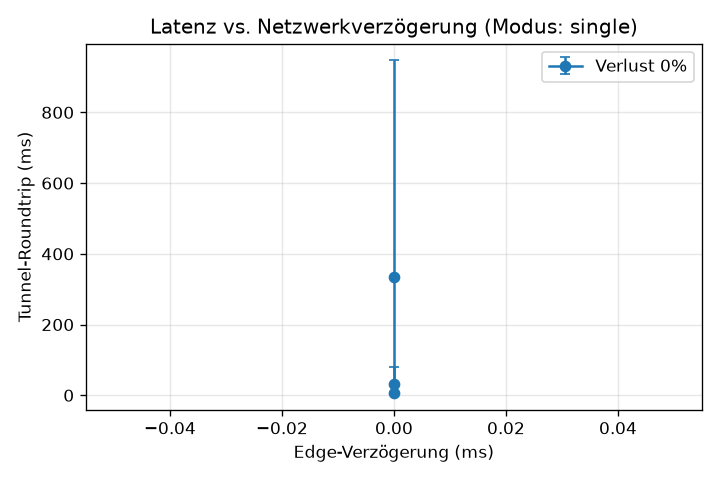
\includegraphics[width=0.8\linewidth]{latency-vs-delay.png}
  \caption{Tunnel-Roundtrip über der Edge-Verzögerung, je Verlustwert eine
    Serie; der obere Fehlerbalken markiert das p95.}
  \label{fig:latency-delay}
\end{figure}

\begin{figure}[t]
  \centering
  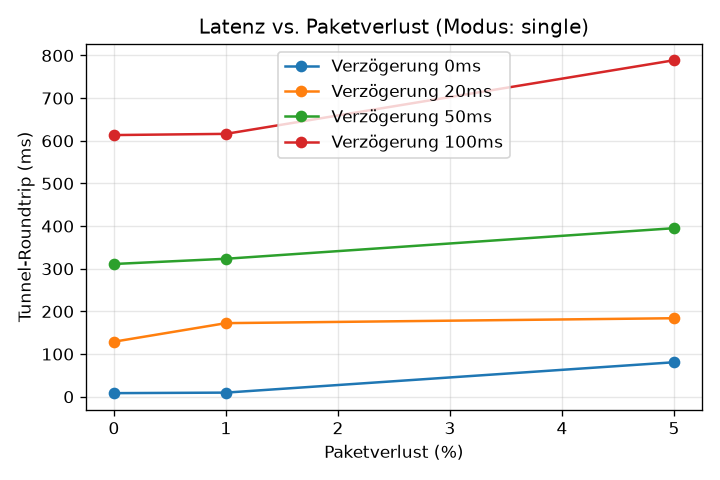
\includegraphics[width=0.8\linewidth]{latency-vs-loss.png}
  \caption{Tunnel-Roundtrip über dem Paketverlust, je Verzögerungswert eine
    Serie.}
  \label{fig:latency-loss}
\end{figure}

\section{Diskussion}
\label{sec:diskussion}

\paragraph{FF2 -- Latenz-Overhead.} Ohne Netzverzögerung beträgt der
Roundtrip im Mittel 6{,}8\,ms; dies ist der Eigenanteil des Tunnels aus
QUIC-Handshake, PoW-Rendezvous und Mehrsprung-Relay. Über die Messpunkte
(0\,ms~$\rightarrow$~6{,}8; 20\,ms~$\rightarrow$~92{,}7; 50\,ms~$\rightarrow$~217{,}9)
skaliert die Latenz näherungsweise linear:
$\text{RT} \approx 6{,}8 + 4{,}2 \cdot d$ mit $d$ = einseitige Edge-Verzögerung
in Millisekunden. Der Faktor~$\approx$~4{,}2 spiegelt wider, dass jeder
Anwendungs-Roundtrip die verzögerte Egress mehrfach quert (Verbindungsaufbau,
Rendezvous und der Relay-Pfad Client$\rightarrow$Edge$\rightarrow$Agent$\rightarrow$Origin
und zurück). Da pro Iteration frisch verbunden wird, trägt der Handshake einen
festen Vielfachen der Umlaufzeit bei.

\paragraph{FF3 -- Verhalten unter Paketverlust.} Bei niedriger Umlaufzeit
(0\,ms, 20\,ms) ist ein Verlust von 2\,\% im Mittel nicht messbar
(6{,}8$\rightarrow$6{,}9\,ms bzw.\ 92{,}7$\rightarrow$92{,}2\,ms, innerhalb der
Streuung). Bei 50\,ms hingegen steigt der Mittelwert um rund 9\,\%
(217{,}9$\rightarrow$237{,}5\,ms) und das p95 um rund 18\,\%
(260{,}4$\rightarrow$306{,}5\,ms), während der Median nahezu unverändert bleibt
(p50~$\approx$~207\,ms). Verlustbedingte Neuübertragungen wirken sich also
proportional zur Umlaufzeit aus und zeigen sich primär im Tail (p95), nicht im
Median.

\section{Limitierungen}
\label{sec:limitierungen}

Die Ergebnisse sind unter drei Einschränkungen zu lesen. Erstens wirkt die
Impairment nur auf der Edge-Egress und damit nicht symmetrisch; die absolute
Latenz ist eine untere Schranke für eine voll bidirektional verzögerte Strecke.
Zweitens dient $n=5$ hier der Demonstration der reproduzierbaren Mess-Pipeline,
nicht einer statistisch belastbaren Aussage -- größere Stichproben und eine
breitere Matrix (inklusive Bandbreitenbegrenzung) sind über dieselben Skripte
unmittelbar zugänglich. Drittens überzeichnet der Frisch-Verbindungsaufbau je
Iteration den Handshake-Anteil; ein Keep-Alive-Datenpfad läge niedriger. Diese
Punkte greift der Ausblick (Kapitel~\ref{ch:fazit}) auf.

\chapter{Fazit und Ausblick}
\label{ch:fazit}

Dieses Kapitel fasst die Ergebnisse zusammen und gibt einen Ausblick. Es wird in
Paket~M7.6 ausgearbeitet und greift die offenen Risiken aus dem Backlog
(\texttt{docs/BACKLOG.md}) auf: Jurisdiktion, Sybil-Resistenz der Abrechnung
sowie Missbrauchsprävention.


% ===================== Anhang / Literatur =====================
\backmatter
\printbibliography[heading=bibintoc]

\end{document}
